\documentclass[11pt,a4paper]{article}

\usepackage{titling}
\usepackage[hidelinks]{hyperref}
\usepackage{graphicx}
\usepackage{grffile}
\usepackage{float}
\usepackage{geometry}
\usepackage{listings}

\newcommand{\subtitle}[1]{
  \posttitle{
    \par\end{center}
    \begin{center}\large#1\end{center}
    \vskip0.5em}
}

\begin{document}
\title{Web Application User Manual}
\subtitle{ Git: \url{https://github.com/CodingInfinity/Benchmark-Service-Documentation} \\ GitHub Organisation: \url{https://github.com/CodingInfinity}}
\begin{figure}
			\centering
			
\includegraphics[height=230px]{../Images/CodingInfinity.png}
\end{figure}
\author{
	\textbf{The Client:} \\
	Ms Vreda Pieterse  \\
	Department of Computer Science \\
	University Of Pretoria
	\\
	\\
	\textbf{The Team:} \\
	Andrew Broekman		\emph{11089777}	\\
	Brenton Watt		\emph{14032644}	\\
	Fabio Loreggian		\emph{14040426}	\\
	Reinhardt Cromhout	\emph{14009936}	\\
}
\date{\textbf{May 2016}}

\maketitle
\thispagestyle{empty}
\pagebreak

\tableofcontents
\pagebreak
\section{Introduction}
This is the user manual for the Web Application. It gives a detailed guide surrounding individual how to
navigate and use each part of the system.

\section{Installation}
Before attempting to use the Web Application, please ensure you have read through and followed the installation
manual for the system as a whole. This can also be found in our repository.

\section{Registration}
Upon starting up of the application and navigating to the home page, the user will be met with the screen seen in 
Figure \ref{fig:landPage}.
\begin{figure}[H]
	\begin{center}
		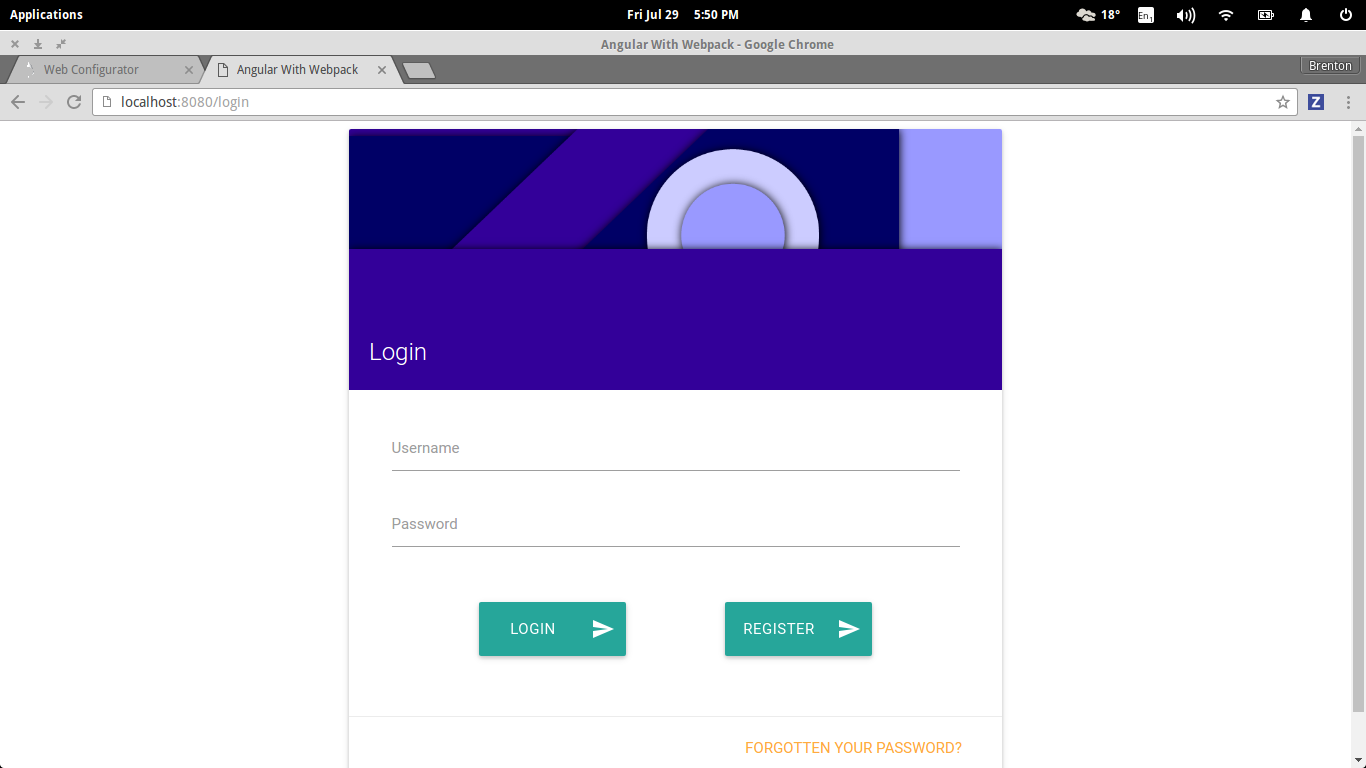
\includegraphics[scale=0.6]{../Images/User Manual/Landing Page.jpg}
		\caption{Landing Page}
		\label{fig:landPage}
	\end{center}  
\end{figure}

If the user has never made use of the system before, they should register themselves. Clicking on the "Register User"
button will direct the user to the page seen in Figure \ref{fig:regPage}.
\begin{figure}[H]
	\begin{center}
		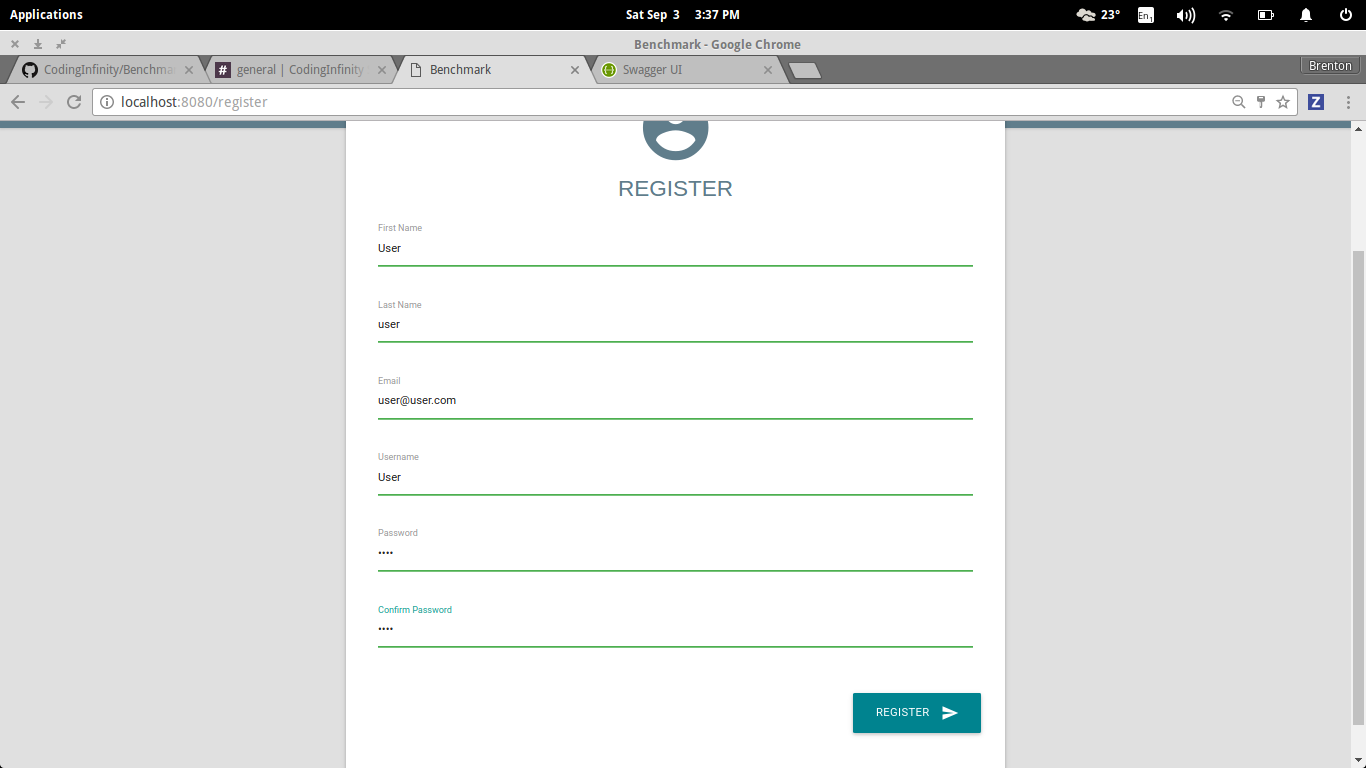
\includegraphics[scale=0.6]{../Images/User Manual/Registration Page.jpg}
		\caption{Registration Page}
		\label{fig:regPage}
	\end{center}  
\end{figure}

The user will then need to fill in their details accordingly. Once they have done this, they should click the "Submit" 
button. The user will then receive an email address at the address provided with a link that will allow them to activate
their account. When they click on the link they will arrive at a page as seen in Figure \ref{fig:activatePage}.
\begin{figure}[H]
	\begin{center}
		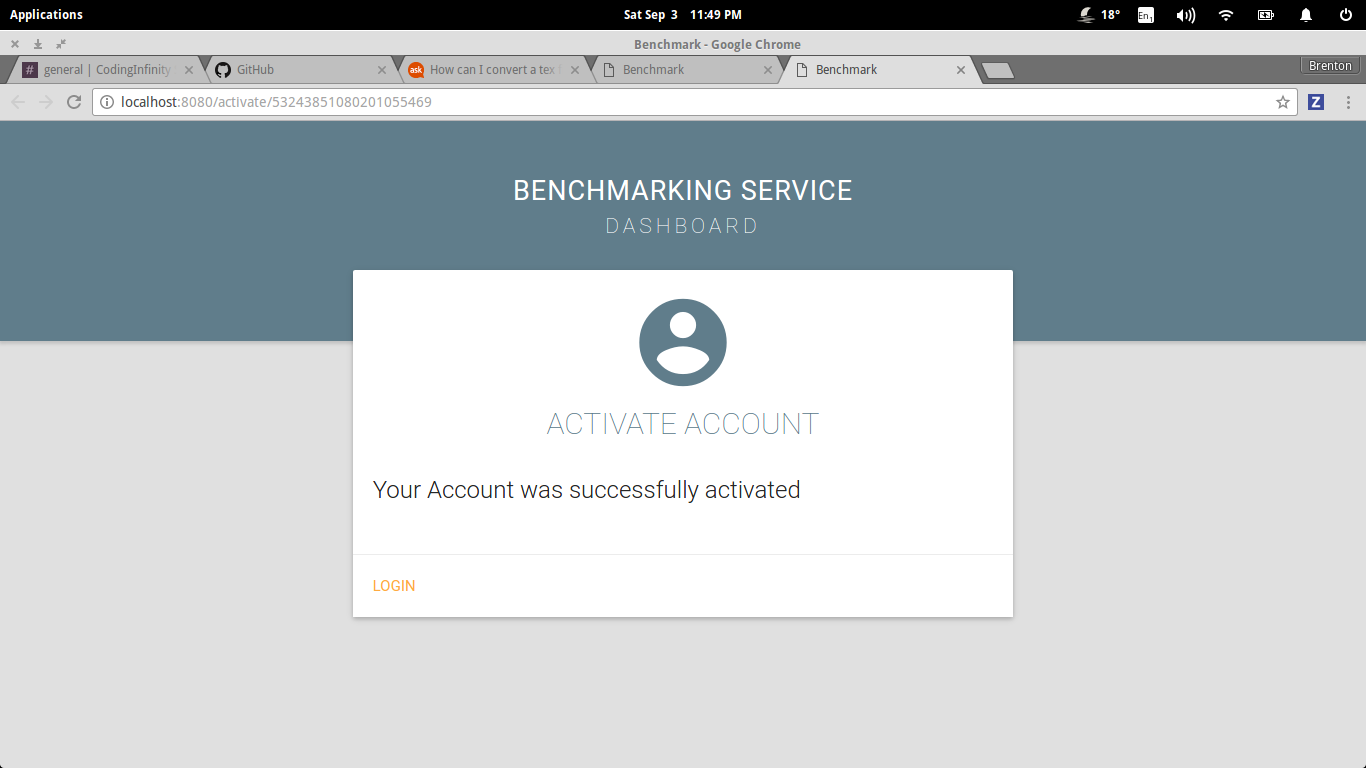
\includegraphics[scale=0.6]{../Images/User Manual/Activation Page.jpg}
		\caption{Activation Page}
		\label{fig:activatePage}
	\end{center}  
\end{figure}

\section{Sign In}
Once the user has registered and activated an account as detailed in the previous section or upon returning to the application,
they will be able to sign in by filling in their details as seen in Figure \ref{fig:signPage}.
\begin{figure}[H]
	\begin{center}
		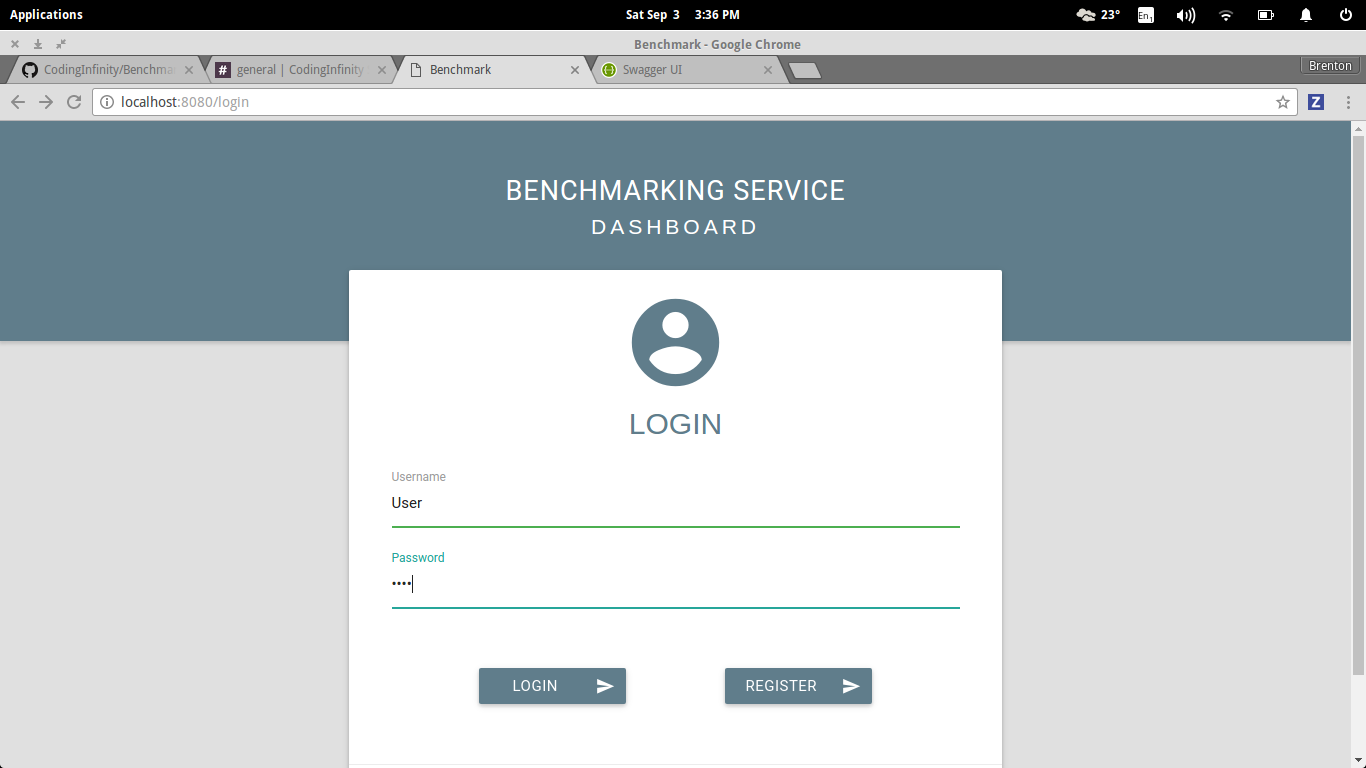
\includegraphics[scale=0.6]{../Images/User Manual/Sign in Page.jpg}
		\caption{Signing in}
		\label{fig:signPage}
	\end{center}  
\end{figure}

\section{Home}
Upon signing in, the user will arrive at the home page as seen in Figure \ref{fig:homePage}. From this page the user will be able 
to navigate throughout the application.
\begin{figure}[H]
	\begin{center}
		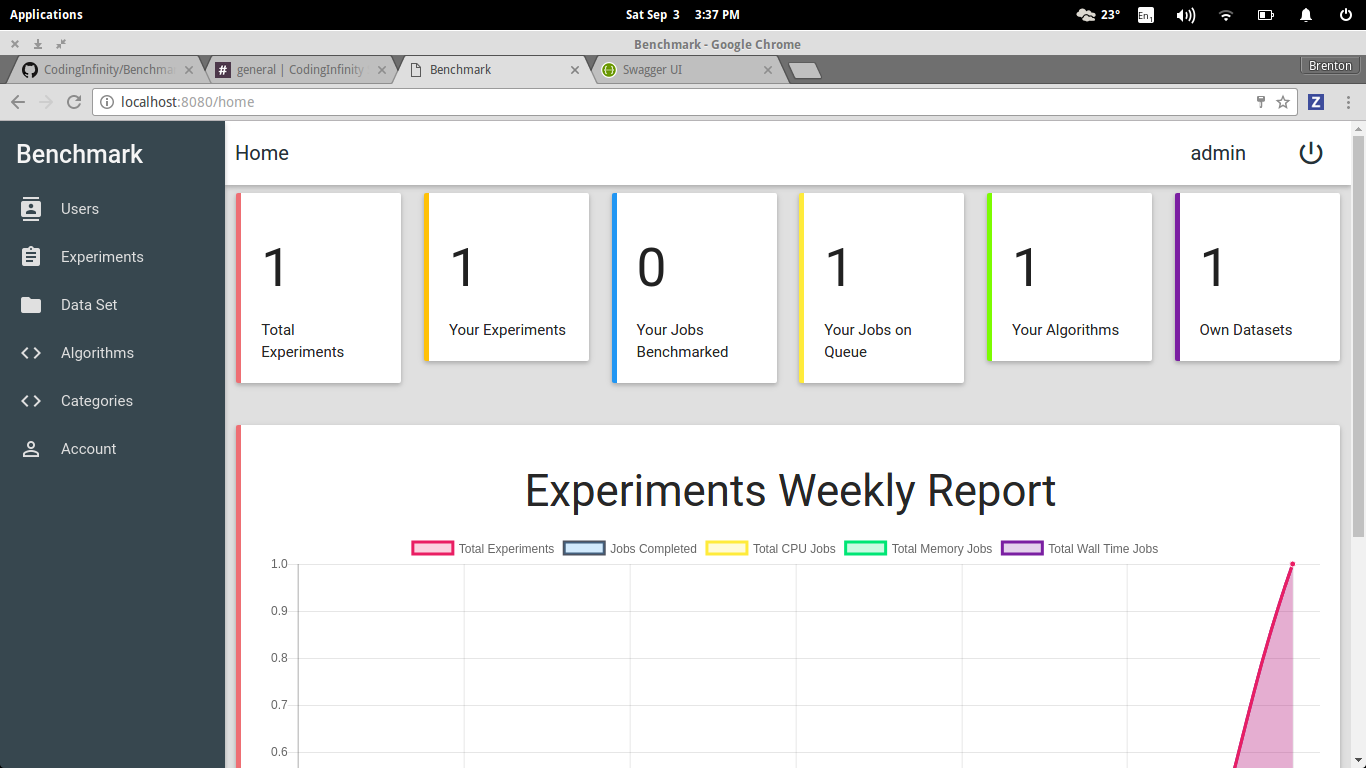
\includegraphics[scale=0.6]{../Images/User Manual/Home Page.jpg}
		\caption{Home Page}
		\label{fig:homePage}
	\end{center}  
\end{figure}
\end{document}